\documentclass[]{article}
\usepackage[utf8]{inputenc}
\usepackage{pdfpages}
\usepackage{amsmath}
\usepackage{amssymb}
\usepackage{graphicx}
\usepackage{geometry}
\usepackage{enumitem}
\usepackage{amsthm}

\usepackage{graphicx}
\usepackage{geometry}

\geometry{hmargin=2cm}

\title{Analyse}

\author{Isabelle Galagher et Pierre Gervais}

% Environnement type théorème
\newtheorem{mythm}{Théorème}
\newtheorem{myproposition}{Proposition}
\newtheorem{myproperty}{Propriété}
\newtheorem{mylemma}{Lemme}
\newtheorem{mycor}{Corollaire}

% Environnement type texte
\theoremstyle{remark}
\newtheorem{mynot}{Notation}
\newtheorem{myrem}{Remarque}
\newtheorem{myexer}{Exercice}
\newtheorem{myproof}{Preuve}
\newtheorem{myexmpl}{Exemple}

% Environnement de définition
\theoremstyle{definition}
\newtheorem{mydef}{Définition}

\setlist[itemize]{label=-}

% Carré de fin de preuve
\newcommand{\cqfd}{
	\hfill$\square$
}

% "Checkmark" de fin d'étape de preuve
\newcommand{\checked}{
	\hfill$\checkmark$
}

% Définition de fonction
\newcommand{\func}[5]{
#1 ~ : ~ \left\{ \begin{array}{lcl}
	#2 & \longrightarrow & #3 \\
	#4 & \longmapsto & #5
\end{array}
\right.
}

\newcommand{\funcinline}[5]{
#1 ~ : ~ #2 \longrightarrow #3, ~ #4 \longmapsto #5
}

\newcommand{\funcshort}[3]{
#1 ~ : ~ #2 \longrightarrow #3
}

\newenvironment{proofpart}[1]{
	\leavevmode
	
	\noindent
	{\textit{\textbf{\boldmath #1}}}
	
}{
	\checkmark
}

\begin{document}

\maketitle

\tableofcontents

\part{Topologie des espaces vectoriels normés}

On considèrera aussi les corps $\mathbb{R}$ ou $\mathbb{C}$

\section{Espaces vectoriels normés : premières définitions}

\subsection{Distances et normes}

\begin{mydef}
	Étant donné un ensemble $E$, une \textit{distance sur $E$} est une application $d~: ~ E \times E \longrightarrow \mathbb{R}$ vérifiant les propriétés suivantes :
	\begin{enumerate}
		\item $d$ est \textit{définie positive} : $d(x,y) \geqslant 0$ et $d(x,y) = 0 \Leftrightarrow x=y$
		\item $d$ est symétrique : $d(x,y)=d(y,x)$
		\item $d$ vérifie l'\textit{inégalité triangulaire} : $\forall z \in E, ~ d(x,y) \leqslant d(x,z) + d(z, y)$
	\end{enumerate}
\end{mydef}

\begin{myexmpl}
	\leavevmode
	\begin{itemize}
		\item $E=\mathbb{R}$ et $d(x, y) = |x-y|$
		\item $E=\mathbb{R}^2$ et $d\left(\binom{a}{b},\binom{c}{d}\right)=\sqrt{(a-c)^2+(b-d)^2}$
	\end{itemize}
\end{myexmpl}

\begin{myrem}
	Par l'inégalité triangulaire, on déduit
	\begin{itemize}
		\item $d(x,z) \geqslant d(x, y) - d(y, z)$
		\item $d(x, z) \geqslant d(z, y) - d(x, y)$
	\end{itemize}
	d'où $|d(x, y) - d(z, y)| \leqslant d(x, z)$
\end{myrem}

\begin{mydef}
	Soit $E$ un $\mathbb{K}$-espace vectoriel, une \textit{norme} sur $E$ est une application notée $N$ ou $\|\cdot\|$ telle que
	\begin{enumerate}
		\item $(x, y) \longmapsto \|x - y\|$ est une distance
		\item $\forall \lambda \in \mathbb{R}, ~ \forall u \in E, ~ \|\lambda u\| = |\lambda|\|u\|$ (\textit{homogénéité})
	\end{enumerate}
\end{mydef}

\begin{myproposition}
	Une fonction $\|\cdot\| ~ : ~ E \longrightarrow \mathbb{R}$ est une norme si et seulement si :
	\begin{enumerate}
		\item elle est homogène
		\item elle est définie
		\item elle vérifie l'inégalité triangulaire
	\end{enumerate}
\end{myproposition}

\begin{myproof}
	\leavevmode
	
	{\boldmath $\Longrightarrow$}
	
	Soit $\|\cdot\|$ une norme.
	\begin{enumerate}
		\item \checkmark
		\item $\|x\|=d(x, 0)$ où $d(x,y)=\|x-y\|$, donc $\|x\| \geqslant 0$ et $\|x\|=0 \Longleftrightarrow d(x, 0)=0 \Longleftrightarrow x=0$
		\item $\|x+y\| = d(x+y, 0) = d(x, -y)$, or $\forall x, y, z \in E, ~ d(x, z) \leqslant d(x, y) + d(y, z)$ donc $d(x, -y) \leqslant d(x, 0) + d(0, -y)$
		D'où $\|x+y\| \leqslant d(x, 0) + d(0, -y) \leqslant \|x\| + \|-y\| \leqslant \|x\| + \|y\|$
	\end{enumerate}
	
	{\boldmath $\Longleftarrow$}
	
	Soit $\| \cdot \|$ vérifiant les trois propriétés, alors soit $d(x, y)=\|x-y\|$ et montrons que d est une distance.
	
	\begin{enumerate}
		\item $d(x, y) \geqslant 0$ car $\|x-y\| \geqslant 0$ par (2).
		$d(x, y) = 0 \Longleftrightarrow \|x-y\| = 0 \Longleftrightarrow x = y$
		
		\item $d(x, y) = \|x-y\|=\|-(x-y)\| = \|y-x\|=d(y, x)$
		
		\item $d(x, y) = \|x-y\| = \|x-z + z - y\| \leqslant \|x-z\| +\|z-x\| \leqslant d(x, y) + d(z, y)$
 	\end{enumerate}
 	\cqfd
\end{myproof}

\begin{myexmpl}
	\leavevmode
	\begin{enumerate}
		\item Dans $\mathbb{R}^n$, on définit les normes $\displaystyle \|x\|_1= \sum_{k=1}^n |x_k|$, $\displaystyle \|x\|_2 =  \sqrt{\sum_{k=1}^n |x_k|^2}$, $\displaystyle \|x\|_p = \sqrt[p]{\sum_{k=1}^n |x_k|^p}$ et $\displaystyle \|x\|_\infty = \max_{k} \|x_k\|$
		\item Dans $\mathbb{R}^n$ muni d'un produit scalaire, $\|x\| = \sqrt{\langle x, x\rangle}$
		\item Soit $A$ un ensemble et $F$ une espace vectoriel normé, et $\mathcal{B}(A, F)$ les fonctions bornées de $A$ dans $F$, alors $\displaystyle \|f\|_\infty = \sup_{x \in A} \|f(x)\|$ est une norme.
		\item Sur $\mathcal{C}([0, 1], \mathbb{R})$, $\displaystyle \|f\|_1 = \int_{0}^{1}\left|f(x)\right|$, $\displaystyle \|f\|_2 = \sqrt{\int_{0}^{1}\left|f(x)\right|^2}$ et$\displaystyle \|f\|_\infty = \sup_{0 \leqslant x \leqslant 1}\left|f(x)\right|$
	\end{enumerate}
\end{myexmpl}

\begin{mydef}
	Deux normes $N_1$ et $N_2$ sont dites \textit{équivalentes} s'il existe des constantes strictement positives $C_1$ et $C_2$ telles que $\forall x \in E, ~ C_1 N_2(x) \leqslant N_1(x) \leqslant C_2 N_2(x)$
\end{mydef}

\begin{myexmpl}
	Par exemple dans $\mathbb{R}^n$, les normes $\|\cdot\|_1$, $\|\cdot\|_2$ et $\|\cdot\|_\infty$ sont équivalentes. En effet $$\|x\|_1=|x_1|+|x_2| \leqslant 2 \|x\|_\infty$$ et $\|x_i| \geqslant \|x\|_\infty, ~ i=1, 2$
\end{myexmpl}

En dimension finie, toutes les normes sont équivalentes ! Cela n'est en revanche pas vraie en dimension infinie.

\begin{figure}[h!]
	\centering
	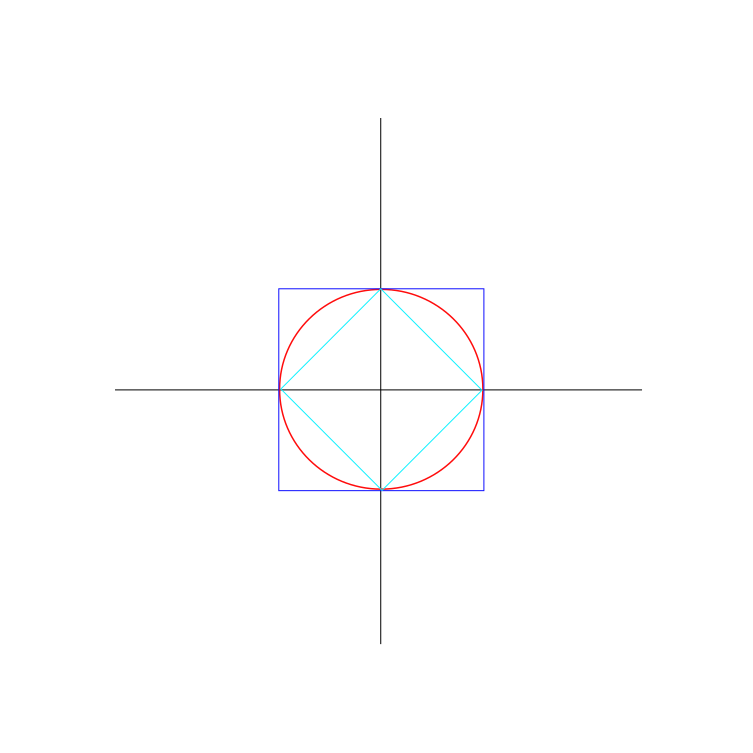
\includegraphics[width=350pt]{Schema1}
	\caption{Différentes boules unités}
	En bleu : $\mathcal{B}_\infty(0, 1)$
	
	En rouge : $\mathcal{B}_2(0, 1)$
	
	En turquoise : $\mathcal{B}_1(0, 1)$
\end{figure}

\subsection{Ouverts et fermés}

\begin{mydef}
	Soit $E$ un espace vectoriel normé, on appelle \textit{boule fermée} de centre $x$ et de rayon $r > 0$ l'ensemble $\overline{\mathcal{B}}(x, r) = \{u \in E ~|~ \|x-u\| \leqslant r\}$, et la \textit{boule ouverte} de centre $x$ et de rayon $r > 0$ l'ensemble $\mathcal{B}(x, r) = \{u \in E ~|~ \|x-u\| < r\}$.
\end{mydef}

\begin{mydef}
	Soit $X \subseteq E$
	\begin{enumerate}
		\item On dit que $U \subseteq X$ est un \textit{ouvert} de $X$ si $\forall x \in U, ~ \exists r > 0 ~ : ~ \mathcal{B}(x, r) \cap X \subseteq U$
		\item On dit que $F \subseteq X$ est un \textit{fermé} de $X$ si son complémentaire dans $X$ est un ouvert de $X$.
	\end{enumerate}
\end{mydef}

\begin{figure}[h!]
	\centering
	\includegraphics[width=200pt]{Ouverts_fermes}	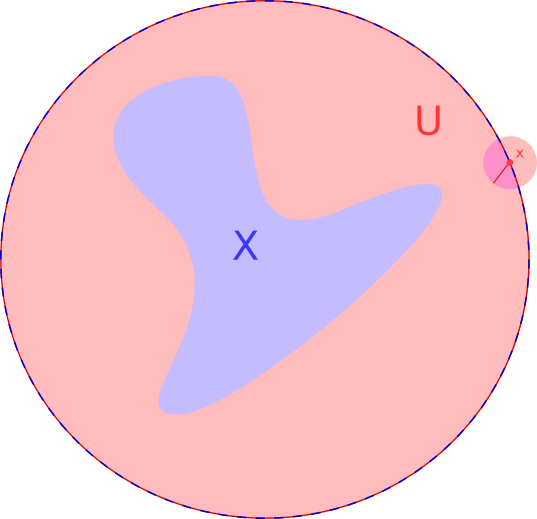
\includegraphics[width=200pt]{Ouverts_fermes2}
	\caption{Deux exemples d'ouverts}
\end{figure}

\begin{myrem}
	\leavevmode
	\begin{enumerate}
		\item Un ouvert dans $X$ n'est pas nécessairement ouvert dans $E$, comme montré dans le deuxième exemple de la figure ci-dessus.
		\item Un ouvert de $E$ sera appelé un \textbf{ouvert}, de même pour les fermés.
		
		\item Toute boule ouverte est un ouvert.
		
		\item Toute boule fermée est un fermé.
	\end{enumerate}
\end{myrem}

\newpage

\begin{myproof}
	On considère une boule ouverte $\mathcal{B}(x_0, r)$, montrons que c'est un ouvert.
	
	Soit $x \in \mathcal{B}(x_0, r)$, alors $\|x-x_0\| < r$. On cherche $r'$ tel que $\mathcal{B}(x, r') \subseteq \mathcal{B}(x_0, r)$ donc $r'$ doit vérifier $$\|x-y\| < r' \Longrightarrow \|x_0-y\| < r$$.
	
	Mais $\|x_0-y\| \leqslant \|x-y\| + \|x-x_0\| < \|x-y\| + r$.
	
	Soit $\delta = r - \|x-x_0\| > 0$, on pose alors $r'=\frac{\delta}{2} > 0$, alors $\|x_0-y\| \leqslant r' + \|x-x_0\| \leqslant r' + r - \delta < r$

	\cqfd
\end{myproof}

\begin{figure}[h!]
	\centering
	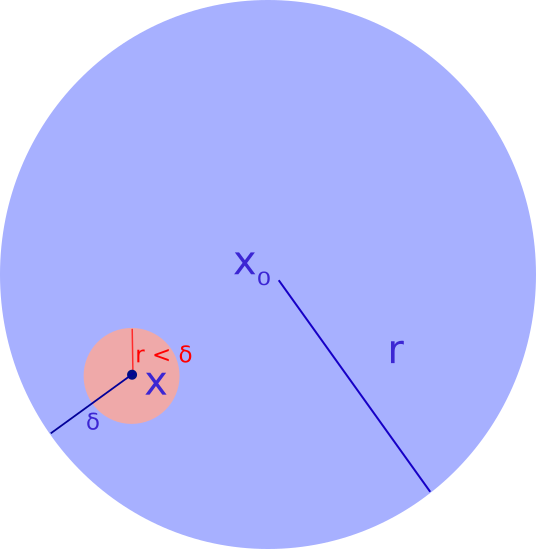
\includegraphics[width=350pt]{Schema2}
	\caption{Construction de la boule ouverte}
\end{figure}

\begin{myproposition}
	L'intersection de deux ouverts est un ouvert et toute réunion d'ouverts est un ouvert.
\end{myproposition}

\begin{myproof}
	Soient $U$ et $U'$ deux ouverts, montrons que $U \cap U'$ est un ouvert.
	
	Soit $x \in U \cap U'$, il existe $r>0$ et $r'>0$ tels que $\mathcal(B)(x, r) \subseteq U$ et $\mathcal{B}(x, r') \subseteq U'$.

	On pose $\widetilde{r}=\min(r, r')$ et on a $\mathcal{B}(x, \widetilde{r}) \subseteq U \cap U'$
	
	\cqfd
\end{myproof}

\begin{myproof}
	Soit $(U_i)_{i \in I}$ une famille d'ouverts, montrons que $U = \displaystyle \bigcup_{i \in I} U_i$ est un ouvert.
	
	Soit $x \in U$, alors il existe $i_0 \in I$ tel que $x \in U_{i_0}$, il existe donc $r$ tel que $\mathcal{B}(x, r) \subseteq U_{i_0}$ car $U_{i_0}$ est ouvert, d'où $\mathcal{B}(x, r) \subseteq U$.
	
	\cqfd
\end{myproof}

\begin{myproposition}
	Soit $X \subseteq E$, tout ouvert $U$ de $X$ s'écrit sous la forme $U=X \cap \widetilde{U}$, où $\widetilde{U}$ est un ouvert.
	
	De même pour tout fermé $F$ de $X$ s'écrit $F=X \cap \widetilde{F}$ où $\widetilde{F}$ est un fermé.
\end{myproposition}

\begin{myproof}
	Soit $\widetilde{U}$ un ouvert de $E$, alors $\widetilde{U} \cap X$ est un ouvert de $X$ par construction.
	
	Inversement soit $U$ ouvert de $X$, alors $\forall x \in U, ~ \exists r(x) > 0$ tel que $\mathcal{B}(x, r(x)) \cap X \subseteq U$
	
	Soit alors $\displaystyle \widetilde{U} = \bigcup_{x \in U} \mathcal{B}(x, r(x))$, alors $\widetilde{U}$ est un ouvert et $U = X \cap \widetilde{U}$
	\cqfd
\end{myproof}

\begin{mydef}
	Une suite à valeurs dans $E$ est dite \textit{convergente vers $x \in E$} si pour tout $\varepsilon > 0$ il existe un rang $N$ tel que pour tout $n \geqslant N$ on ait $\|x_n-x\| < \varepsilon$.
	
	Celle-ci est unique et on la note $\lim\limits_{n} x_n = x$.
\end{mydef}

On remarquera qu'une suite convergente est bornée.

\begin{myproof}
	Soient $x$ et $y$ deux limites de la suite convergente $(x_n)_n$.
	
	Pour tout $\varepsilon > 0$ on peut trouver un rang $N$ à partir duquel $\|x_n-x\|<\varepsilon$ et $\|y_n-x\|<\varepsilon$, d'où
	
	$$\|x-y\| \leqslant \|x-x_n\| + \|x_n-y\| < 2\varepsilon$$
	
	Cette inégalité est vraie pour tout $\varepsilon>0$ donc $x=y$.
	
	\cqfd
\end{myproof}

\begin{myrem}
	On rappelle que dans $\mathbb{R}$, toute suite majorée croissante est convergente.
	
	Soit $A=\{x_n ~ | ~ n \geqslant 0\}$, et on note $l = \sup A$.
	
	Soit $\varepsilon > 0$, $l - \varepsilon$ ne majore pas $A$ donc il existe un rang $N$ à partir duquel $x_n \geqslant l-\varepsilon$, mais on a aussi $x_n \leqslant l$ pour tout $n$, on a ainsi à partir de $N$ l'encadrement $l - \varepsilon \leqslant x_n \leqslant l + \varepsilon$.
	
	On a de plus que $\lim\limits_{n} x_n = \sup \{x_n | n \geqslant 0\}$
\end{myrem}

\begin{myrem}
	Si une suite est convergente pour une norme, alors elle l'est pour toute norme équivalente à celle-ci.
	
	Cela n'est pas vrai en général si les normes ne sont pas équivalentes.
	
	Sur l'ensemble des fonctions continue sur $[0, 1]$ on définit les normes
	
	$$\|f\|_{\infty} = \sup_{[0,1]} |f(x)| \text{ et } \|f\| = \int_{0}^{1} |f|$$
	
	On considère la suite de fonction $f_n ~ : ~ x \longmapsto x^n$, on a $$\displaystyle \|f_n\|_{\infty} = \sup_{[0, 1]} |f_n(x)| = 1$$ mais $\|f_n\|=\int_{0}^{1}x^ndx=\frac{1}{n+1} \longrightarrow 0$, les normes ne sont pas équivalentes.
\end{myrem}

\begin{mydef}
	On appelle \textit{valeur d'adhérence} de $x_n$ toute limite d'une sous-suite (suite extraite) de $(x_n)$.
	
	Et on appelle \textit{point d'accumulation} d'une suite $(x_n)$ un point $x$ tel que $\forall \varepsilon > 0, ~ \forall N, ~ \exists n > N ~ : ~ \|x_n-x\| < \varepsilon$.
\end{mydef}

\begin{myproposition}
	Tout point d'accumulation d'une suite convergente $(x_n)$ est une valeur d'adhérence, et réciproquement.
\end{myproposition}

\begin{myproof}
	\begin{proofpart}{Valeur d'adhérence $\Longrightarrow$ point d'accumulation :}
	
		Soit $x$ une valeur d'adhérence de $(x_n)$, il existe une fonction entière strictement croissante $\varphi$ telle que $$\forall \varepsilon > 0, ~ \exists N ~ : ~ \forall n > N, ~ \|x_{\varphi(n)}-x\| < \varepsilon$$
		donc $x$ est un point d'accumulation.
	\end{proofpart}
	
	\begin{proofpart}{Point d'accumulation $\Longrightarrow$ valeur d'adhérence :}
		Réciproquement, soit $x$ un point d'accumulation d'une suite $(x_n)$, on construit par récurrence $\varphi$ telle que $x$ soit la limite de $(x_{\varphi(n)})_n$ par 
		
		$$
		\varphi(n) = \left\{
			\begin{array}{ll}
				0, ~ n = 0 \\
				\min\{k > \varphi(n-1) ~ | ~ \|x_k-x\| < 2^{-n}\}, ~ n > 0
			\end{array}
		\right.
		$$
		
		L'application est bien strictement croissante.
		
		Montrons à présent que $y_n=x_{\varphi(n)}$ converge vers $x$ : 
		
		soit $\varepsilon \in ]0, 1[$, on cherche $N$ tel que pour tout $n > N, ~ \|x_n-x\| < \varepsilon$.
		
		Pour $N > \frac{\ln \varepsilon}{\ln 2}$ on a $$\forall n > N, ~ \|y_n-x\| < 2^{-n} < \varepsilon$$
		
		$(y_n)_n$ est bien une suite convergeant vers $x$.
	\end{proofpart}
	
\end{myproof}

\begin{myproposition}
	Soit $E$ un espace vectoriel normé et $F \subseteq E$.
	
	F est fermé \textit{si et seulement si} $F$ contient la limite de toutes ses suites convergentes.
\end{myproposition}

\begin{myproof}
	\begin{proofpart}{$F$ fermé $\Longrightarrow$ $F$ contient les limites de ses suites}

		Soit $(x_n)$ une suite convergente de $F$ de limite $x$. Montrons que $x \in F$.
		
		Supposons par l'absurde $x \not \in F$, alors $x \in F^C$ qui est ouvert. Il existe donc $r > 0$ tel que $\mathcal{B}(x, r) \subseteq (E \verb|\|F)$, mais il existe un rang à partir duquel $\|x_n-x\| < \frac{r}{2}$, c'est à dire $x_n \in \mathcal{B}(x, r)$, ce qui contredit $\mathcal{B}(x, r) \subseteq F^C$.
	\end{proofpart}
	
	
	\begin{proofpart}{$F$ contient les limites de ses suites $\Longrightarrow$ $F$ est fermé}
		Montrons que $F^C$ est fermé, ce qui est est équivalent au fait que $F$ soit fermé.
		Soit $u \in F^C$, on pose $r=\inf\limits_{f \in F} \|f-u\|$.
		
		Supposons par l'absurde que $r$ soit nul, alors pour tout $n>0$ il existerait un élément $f_n \in F$ tel que $\|u-f_n\| < \frac{1}{n}$. Cela définit alors une suite $(f_n)_n$ à valeurs dans $F$ convergente vers $u \notin F$, ce qui contredit le fait que $F$ contienne ses limites.
		
		On a alors $\mathcal{B}_r(u) \subseteq F^C$, $F^C$ est donc effectivement ouvert.
	\end{proofpart}
	\begin{figure}[h!]
		\centering
		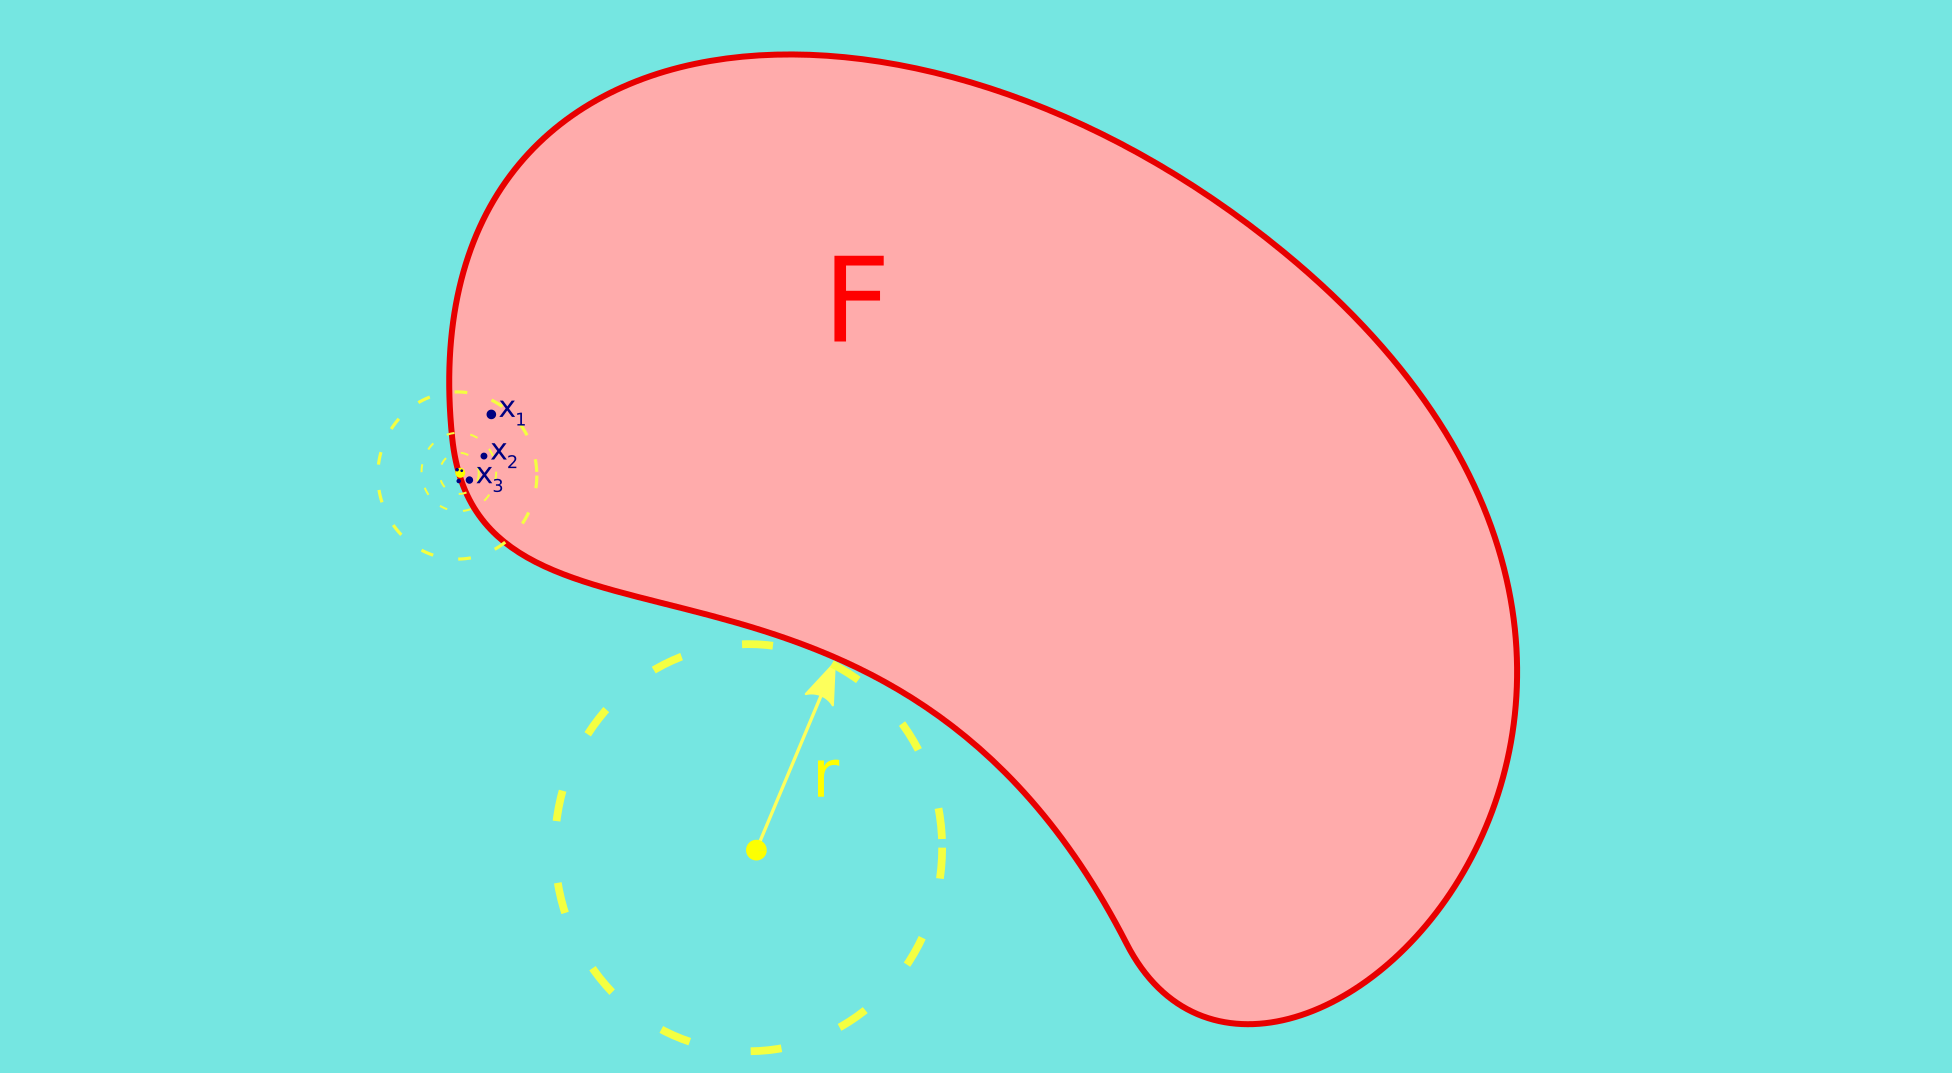
\includegraphics[width=450pt]{Contient_ses_limites_implique_ferme}
		\caption{Une partie contenant ses limites est fermée}
		
		Si on avait $r=\inf\limits_{f \in F} \|u-f\|=0$, alors on aurait $u \in F$ car toute boule ouverte centrée en $u$ s'intersecterait avec le fermé $F$. 
	\end{figure}	
	\cqfd
\end{myproof}

\begin{mydef}
	Soit $X$ une partie d'un espace vectoriel normé $E$.
	
	\begin{itemize}
	\item \textit{L'intérieur de $X$} est le plus grand ouvert inclus dans $X$ noté $\mathring{A}$.
	
	\item \textit{L'adhérence de $X$} est le plus petit fermé contenant $X$ noté $\overline{X}$.
	
	\item \textit{La frontière de $X$} est l'ensemble $\partial X=Fr(X)=\overline{X} \verb|\| \mathring{X}$
	\end{itemize}
\end{mydef}

\begin{myexmpl}
	Si $X = ]0, 1]$ sur $\mathbb{R}$ alors $\mathring{X} = ]0, 1[$, $\overline{X}=[0, 1]$ et $Fr(X)=\{0, 1\}$.
\end{myexmpl}

\begin{myrem}
	X est ouvert si est seulement si $\mathring{X} = X$ et $X$ est fermé si et seulement si $\overline{X}=X$.
	
	En effet, pour $X$ ouvert, $\mathring{X}$ est le plus grand ouvert contenu dans $X$, donc $X$.
	
	Réciproquement si $X=\mathring{X}$, l'intérieur d'une partie étant un ouvert on a bien que $X$ est ouvert.
\end{myrem}

\begin{myproof}Intérieur
	
	Soit $\mathring{X}$ l'ensemble des $x \in X$ tels qu'il existe $r > 0$ tel que $\mathcal{B}(x, r) \subseteq X$, alors $\mathring{X}$ est la réunion de tous les ouverts contenus dans $X$.
	
	En effet, $\mathring{X}$ est ouvert dans $X$ par définiton, donc $\mathring{X} \subseteq \text{"réunion des ouverts de X"}$.
	
	Soit $U$ un ouvert de $X$, montrer que $U \subseteq X$.
	
	Soit $x \in U$, il existe $r>0$ tel que $\mathcal{B}(x, r) \subseteq U$ ar $U$ est ouvert. Donc $x \in \mathring{X}$.
	
	$\mathring{X}$ est donc ouvert, contenu dans $X$. Il contient tous les ouverts de $X$, donc c'est le plus grand de $X$, d'où le résultat.
	\cqfd
\end{myproof}

\begin{myproposition}
	On caractérise l'adhérence d'une partie $X$ comme étant l'ensemble des limites de sous-suites de $X$.
\end{myproposition}

\begin{myproof}
	Soit $A$ l'ensemble des limites de suites convergentes à valeurs dans $X$.
	
	
	\begin{proofpart}{$A$ est un fermé contenant $X$}
		Pour tout $x \in X$, $x$ peut être la limite d'une suite à valeur dans $X$, c'est à dire $x \in A$ et donc $X \subseteq A$.
		
		Cela signifie en particulier que $A$ contient les limites de ses suites : c'est un fermé.
	\end{proofpart}
	
	\begin{proofpart}{$A$ est le plus petit fermé contenant X}
	
	Montrons que $A$ est minimal, c'est-à-dire que pour tout fermé $F$ vérifiant $X \subseteq F \subseteq A$, on a $F=A$.
	
	$F$ est un fermé contenant $X$, donc il contient $X$ et les limites des suites convergentes à valeurs dans $X$, c'est à dire $A$.
	\end{proofpart}
	
	$A$ est donc le plus petit fermé contenant $X$, c'est à dire $A = \overline{X}$	
\end{myproof}

\section{Applications continues}

\begin{mydef}
	Soient $E$ et $F$ deux espaces vectoriels normés, soient $X \subseteq E$, $Y \subseteq F$ et $f$ une application de $X$ dans $Y$.
	
	On dit que $f$ est continue en un point $x \in X$ si $$\forall \varepsilon > 0, \exists \delta > 0 ~ : ~ (\forall u, ~ \|x-u\| < \delta \Longrightarrow \|f(x)-f(u)\| < \varepsilon)$$
\end{mydef}

\begin{mythm}
	Une application $f~:~X \longrightarrow Y$ est continue en $x_0 \in X$ si et seulement si pour toute suite $(y_n)$ convergeant vers $x_0$, la suite $\left(f(y_n)\right)_n$ converge vers $f(x_0)$.
\end{mythm}

\begin{myexer}
	Le démontrer
\end{myexer}

\begin{mythm}
	Soit une application $f~:~X \longrightarrow Y$, les assertions suivantes sont équivalentes :
	\begin{enumerate}
	 \item $f$ est continue sur $X$
	 \item l'image réciproque de tout ouvert de $Y$ est un ouvert de $X$
	 \item l'image réciproque de tout fermé de $X$ est une fermé de $X$.
 	\end{enumerate}
\end{mythm}

\begin{myproof}
	\begin{proofpart}{1. $\Longrightarrow$ 2.}
		Soit $f$ continue sur $X$ et $U$ un ouvert de $Y$. Montrer que $f^{-1}(U)=V$ est un ouvert de $X$.
		
		Soit $x \in f^{-1}(U)$, alors $f(x) \in U$, il existe donc $r>0$ tel que $\mathcal{B}(f(x), r) \subseteq U$.
		
		Or il existe $\delta > 0$ tel que pour $\|x-u\| < \delta$, on a $\|f(x)-f(y)\| < \frac{r}{2}$.
		
		Ainsi si $y \in \mathcal{B}\left(x, \frac{\delta}{2}\right)$ alors $f(y) \in \mathcal{B}(f(x), r) \subseteq U$, donc $y \in f^{-1}(U)$.
		
		$f^{-1}(U)$ est donc un ouvert.
	\end{proofpart}
	
	\begin{proofpart}{2. $\Longrightarrow$ 1.}
		Soit $\varepsilon > 0$, on veut trouver $\delta > 0$ tel que si $\|x-y\| < \delta$, alors $\|f(x)-f(y)\| < \varepsilon$.
	
		Soit $x \in X$, alors $\mathcal{B}_\varepsilon(f(x))$ est un ouvert de de $Y$, on sait que $f^{-1}(\mathcal{B}_\varepsilon(f(x)))$ est un ouvert de $X$ contenant $x$, il existe donc $\delta > 0$ tel que $\mathcal{B}_\delta(x) \subseteq f^{-1}(\mathcal{B}_\varepsilon(f(x)))$.
		
		Autrement dit, si $\|x-y\| < \delta$ alors $y \in f^{-1}(\mathcal{B}_\varepsilon(f(x)))$, c'est-à-dire $\|f(x)-f(y)\| < \varepsilon$.
	\end{proofpart}
	
	\begin{proofpart}{1. $\Longleftrightarrow$ 2.}
		On le démontre en passant au complémentaire.
	\end{proofpart}
	
	\cqfd
\end{myproof}

\begin{mycor}
	Soient $X \subseteq E$, $Y \subseteq F$ et $f$ une application de $X$ dans $Y$.
	\begin{enumerate}
		\item On suppose que $f$ est continue, alors la restriction de $f$ à $X' \subseteq X$ notée $f_{|X'}$ est continue.
		
		\item Si $X'$ est un ouvert de $X$ et si $f_{|X'}$ est continue alors $f$ est continue en tout point de $X'$.
		
		\item Soient $f$ et $g$  avec $\funcshort{f}{E}{F}$ et $\funcshort{g}{F}{G}$ avec $E, F, G$ des espaces vectoriels normés. Si $f$ et $g$ sont continues alors $g \circ f$ est continue.
	\end{enumerate}
\end{mycor}

\newpage

\begin{myrem}
	L'hypothèse que $X'$ soit ouvert est nécessaire pour le point 2.
	\begin{figure}[h!]
		\centering
		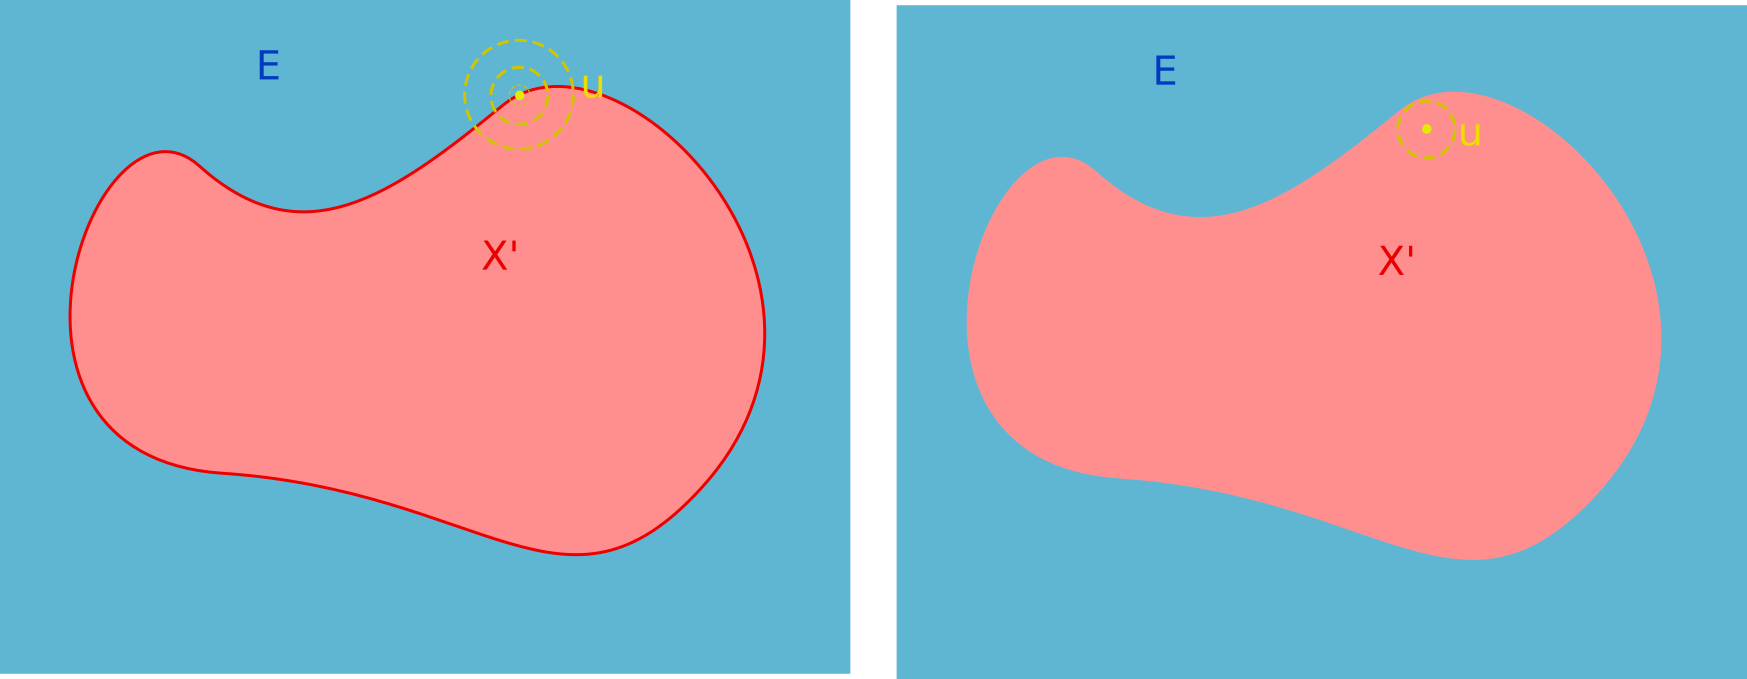
\includegraphics[width=550pt]{Application_continue}
		\caption{Restriction continue sur une partie non-ouverte ou ouverte}
		
		$\func{f}{\mathbb{R}^2}{\mathbb{R}}{u}{\text{rouge si } u \in X', ~ \text{ bleu sinon}}$
		
		\begin{itemize}
		\item A gauche, $f_{|X'}$ est continue mais $f$ n'est pas continue sur $X'$ car on ne peut pas trouver une boule ouverte de $X'$ autour du point $u$.
		
		\item A droite, on peut trouver une boule ouverte autour de $u$ car $X'$ est ouvert.
		\end{itemize}
	\end{figure}
\end{myrem}

\begin{myproof}
	\begin{proofpart}{Point 1.}
		Soit $X' \subseteq X$ et $V$ un ouvert de $Y$, montrons que $\left(f_{|X'}\right)^{-1}(V)$ est un ouvert de $X'$.
		
		$f$ est continue sur donc il existe $U$ ouvert de $E$ tel que $f^{-1}(V)= X \cap U$.
		
		Mais alors $\left(f_{|X'}\right)^{-1}(V) = X' \cap X \cap U = X' \cap U$ qui est un ouvert de $X'$.
		
		Donc $f_{|X'}$ est continue.
	\end{proofpart}
	
	\begin{proofpart}{Point 2.}
		$f_{|X'}$ est continue, soit $x \in X'$, montrons que $f$ est continue en $x$.
		
		Soit $\varepsilon > 0$, il existe $\delta
		 > 0$ tel que si $y \in X'$ et $\|x-y\| < \delta$ alors $\|f(x)-f(y)\| < \varepsilon$
		 
		 Comme $X'$ est ouvert, il existe $r > 0$ tel que $\mathcal{B}_r(x) \subseteq X'$.
		 
		 On choisit $\delta' \leqslant \min\{r, \delta\}$, alors $\forall y \in \mathcal{B}_{\delta'}, ~ \|f(x)-f(y)\| < \varepsilon$, donc $f$ est continue en $x$.
	\end{proofpart}
	
	\begin{proofpart}{Point 3.}
	\end{proofpart}
\end{myproof}


\section{Applications uniformément continues, applications linéaires continues}

\begin{mydef}
	Une application $\funcshort{f}{E}{F}$ est \textit{uniformément continue} si $$\forall \varepsilon, ~ \exists \delta > 0 ~ : ~ \forall x, y \in E, ~ (\|x-y\| < \delta \Longrightarrow \|f(x)-f(y\| < \varepsilon)$$
\end{mydef}

\begin{myrem}
	Si est uniformément continue alors elle est continue, la réciproque ets cependant fausse.
\end{myrem}

\begin{mydef}
	Une fonction $f$ est $k$-\textit{lipschitzienne} si
	
	$$\forall x, y \in E, ~ \|f(x)-f(y)\| \leqslant k \|x-y\|$$
\end{mydef}

\begin{mythm}
	Soit $\funcshort{\varphi}{E}{F}$ une application linéaire, alors les propriétés suivantes ont équivalentes :
	
	\begin{enumerate}
		\item $\varphi$ est continue
		\item $\varphi$ est continue en 0
		\item $\varphi$ est uniformément continue
		\item $\varphi$ est bornée sur $\mathcal{B}_1(0)$
		\item $\varphi$ est $k$-lipschitzienne.
	\end{enumerate}
\end{mythm}


\begin{myproof}
	Montrons $2. \Longrightarrow 4. \Longrightarrow 5. \Longrightarrow 3.\Longrightarrow 1. \Longrightarrow 2.$
	
	\begin{proofpart}{$1. \Longrightarrow 2.$}
	\end{proofpart}
	
	\begin{proofpart}{$2. \Longrightarrow 4.$}
		$f$ est continue en 0, donc pour tout $\varepsilon > 0$ il existe $\delta > 0$ tel que $\|x\| < \delta \Longrightarrow \|f(x)\| < \varepsilon$
		
		Soit $x \in \mathcal{B}_1(0)$ avec $x \neq 0$, on a :
		
		$$\|x\| < 1$$

		$$\|\delta x\| < \delta$$
		
		$$\|f(\delta \cdot x)\| < \varepsilon$$
		
		$$\|f(x)\| < \frac{\varepsilon}{\delta}$$
	\end{proofpart}
	
	\begin{proofpart}{$4. \Longrightarrow 5.$}
		Supposons que $f$ soit majoré par $M > 0$ sur la boule unité.
		
		Soient $x \neq y \in E$, on a
		$$x-y = (x-y) \cdot \frac{\|x-y\|}{\|x-y\|}$$
		
		$$f(x-y) = \|x-y\| f\underbrace{\left(\frac{x-y}{\|x-y\|}\right)}_{\in \mathcal{B}_1(0)}$$
		
		$$f(x-y) = \|x-y\| \cdot M$$
		
		$f$ est $M$-lipschitzienne.
	\end{proofpart}
	
	\begin{proofpart}{$5. \Longrightarrow 3. \Longleftarrow 1. \Longrightarrow 2.$}
	\end{proofpart}
\end{myproof}

\begin{mydef}
	Soit $f$ une application lipschitzienne, on appelle \textit{constante de Lipschitz de $f$} ou \textit{norme d'opérateur de $f$} la valeur $\|f\| = \inf \{k > 0 ~|~ f \text{ est }k \text{-liptschitzienne}\} = \sup\limits_{\|x\|=1} \|f(x)\| = \sup\limits_{\|x\| \leqslant1} \|f(x)\|$
\end{mydef}

La norme d'opérateur est comme son nom l'indique une norme, en particulier $$\forall x, y \in E, ~ \|f(x)\|\leqslant \|f\|\|x\|$$

\begin{myproposition}
	Soient $E$ et $F$ deux espaces vectoriels normés, o note $\mathcal{L}_C(E)$ l'ensemble des applications linéaires continues de $E$ dans $F$. C'est un espace vectoriel normé si on le munit de la norme d'opérateur.
	
	$$\forall \varphi, \psi \in \mathcal{L}_C(E, E), ~ \|\varphi \circ \psi\| \leqslant \|\varphi\| \|\psi\|$$
\end{myproposition}

\begin{myrem}
	On peut étendre ces résultats aux applications bilinéaires : soient $E$, $E'$ et $F$ trois espaces vectoriels normés, et $\funcshort{f}{E \times E'}{F}$ bilinéaire continue,sa norme d'opérateur est définie par
	$$\|f\| = \sup\{\|f(x, y)\| ~ | ~ \|x\| \leqslant 1, ~ \|y\| \leqslant 1\}$$
	
	On a en particulier $\|f(x,y)\| \leqslant \|f\| \cdot \|x\| \cdot \|y\|$
\end{myrem}

\section{Espaces produits}

\begin{mydef}
	Soient $(E_1, N_1)$ et $(E_2, N_2)$ deux espaces vectoriels normés, on construit des normes sur $E_1 \times E_2$ en posant
	$$\|(x, y)\|_1 = N_1(x) + N_2(y)$$
	$$\|(x, y)\|_2 = \sqrt{N_1^2(x) + N_2^2(y)}$$
	$$\|(x, y)\|_\infty = \max\{N_1(x), N_2(y)\}$$
\end{mydef}

On a les relations $$\|(x, y)\|_\infty \leqslant \|(x, y)\|_2 \leqslant \|(x, y)\|_1 \leqslant 2 \|(x, y)\|_\infty$$

\begin{myexmpl}
	Soit $E$ un espace vectoriel normé, on munit $E \times E$ de la norme définie par $N(x, y)=\|x\|+\|y\|$ et on définit une distance $d(u, v)=\|u-v\|$
	
	$d$ est lipschitzienne :
	$$|d(x, y) - d(x', y')|=|\|x-y\|-\|x'-y'\||$$
	
	$$|d(x, y) - d(x', y')| \leqslant |\|(x-y)-(x'-y')\||$$
	
	$$|d(x, y) - d(x', y')| \leqslant |\|(x-x')+(y'-y)\||$$

	$$|d(x, y) - d(x', y')| \leqslant \|(x-x')\|+\|(y'-y)\|$$
	
	$$|d(x, y) - d(x', y')| \leqslant N((x-x')+(y'-y))$$
	
	$d$ est donc 1-lipschitzienne.
\end{myexmpl}

\begin{myproposition}
	Soient $E_1$ et $E_2$ deux espaces vectoriels normés, alors :
	
	\begin{enumerate}
		\item Les projections $\func{\pi_1}{E_1 \times E_2}{E_1}{(x,y)}{x}$
		et $\func{\pi_2}{E_1 \times E_2}{E_1}{(x,y)}{y}$
		sont lipschitziennes.
		
		\item Une application $\funcshort{f}{Y}{E_1 \times E_2}$ notée $f=(f_1, f_2)$ avec $\funcshort{f_1}{Y}{E_1}$ et $\funcshort{f_2}{Y}{E_2}$ est continue si et seulement si $f_1$ et $f_2$ sont continues.
		
		\item Si $\funcshort{f}{E_1 \times E_2}{F}$ est continue alors pour tout $x \in E_1$, l'application $\func{f_x}{E_2}{F}{y}{f(x, y)}$ est continue et de même $\func{f_y}{E_1}{F}{x}{f(x, y)}$ est continue pour tout $y \in E_2$.
	\end{enumerate}
\end{myproposition}

\begin{myproof}
	\begin{enumerate}
		\item Soit $(x, y) \in E_1 \times E_2$, alors $\pi_1(x, y) = x$, donc $\pi_1(x,y) - \pi_2(x',y')=x'-y'$ et donc $\|\pi_1(x,y) - \pi_2(x',y')\| = \|x-x'\| \leqslant \|x-x'\| + \|y-y'\| = N_1(x-x', y-y')$
		
		$\pi_1$ est 1-lipschitzienne.
		
		\item Si $f$ est continue, alors $\pi_1 \circ f=f_1$ est continue comme composée d'applications continues.
		
		De même $f_2=\pi_2 \circ f$ est continue.
		
		Inversement, supposons que $\funcshort{f_1}{Y}{E_1}$ et $\funcshort{f_2}{Y}{E_2}$ sont continues.
		
		Montrons que $\func{f=(f_1, f_2)}{Y}{E \times E_2}{x}{(f_1(x), f_2(y)}$
		
		Soit $(x_n)_n$ une suite de $Y$ convergeant vers $x \in Y$, montrons que $(f(x_n))_n$ converge vers $f(x)$.
		
		Comme $f_1$ est continue, $(f_1(x_n))_n$ converge $f_1(x)$ et de même pour $f_2$.
		
		Donc $f(x_n)_n$ converge vers $f(x)=(f_1(x), f_2(x))$
		
		\item Se démontre de même par caractérisation séquentielle de la continuité.
	\end{enumerate}
\end{myproof}

\begin{myrem}
	Une fonction peut être continue de chaque variable sans être continue du couple de variables, par exemple
	$$f ~ : ~ \left\{
	\begin{array}{ccl}
		\mathbb{R}^2 & \longrightarrow & \mathbb{R} \\
		(x, y) & \longmapsto & \frac{xy}{x^2+y^2}, \text{ si } (x, y) \neq (0, 0) \\
		(0, 0) & \longmapsto & 0
	\end{array}
	\right.$$
	
	$f$ est continue pour $x$ et $y$ fixé, mais $\forall \varepsilon > 0, ~ f(\varepsilon, \varepsilon) = \frac{1}{2}$
	$f$ n'est donc pas continue car $f(0, 0)=0$.
	
		\begin{figure}[h!]
			\centering
			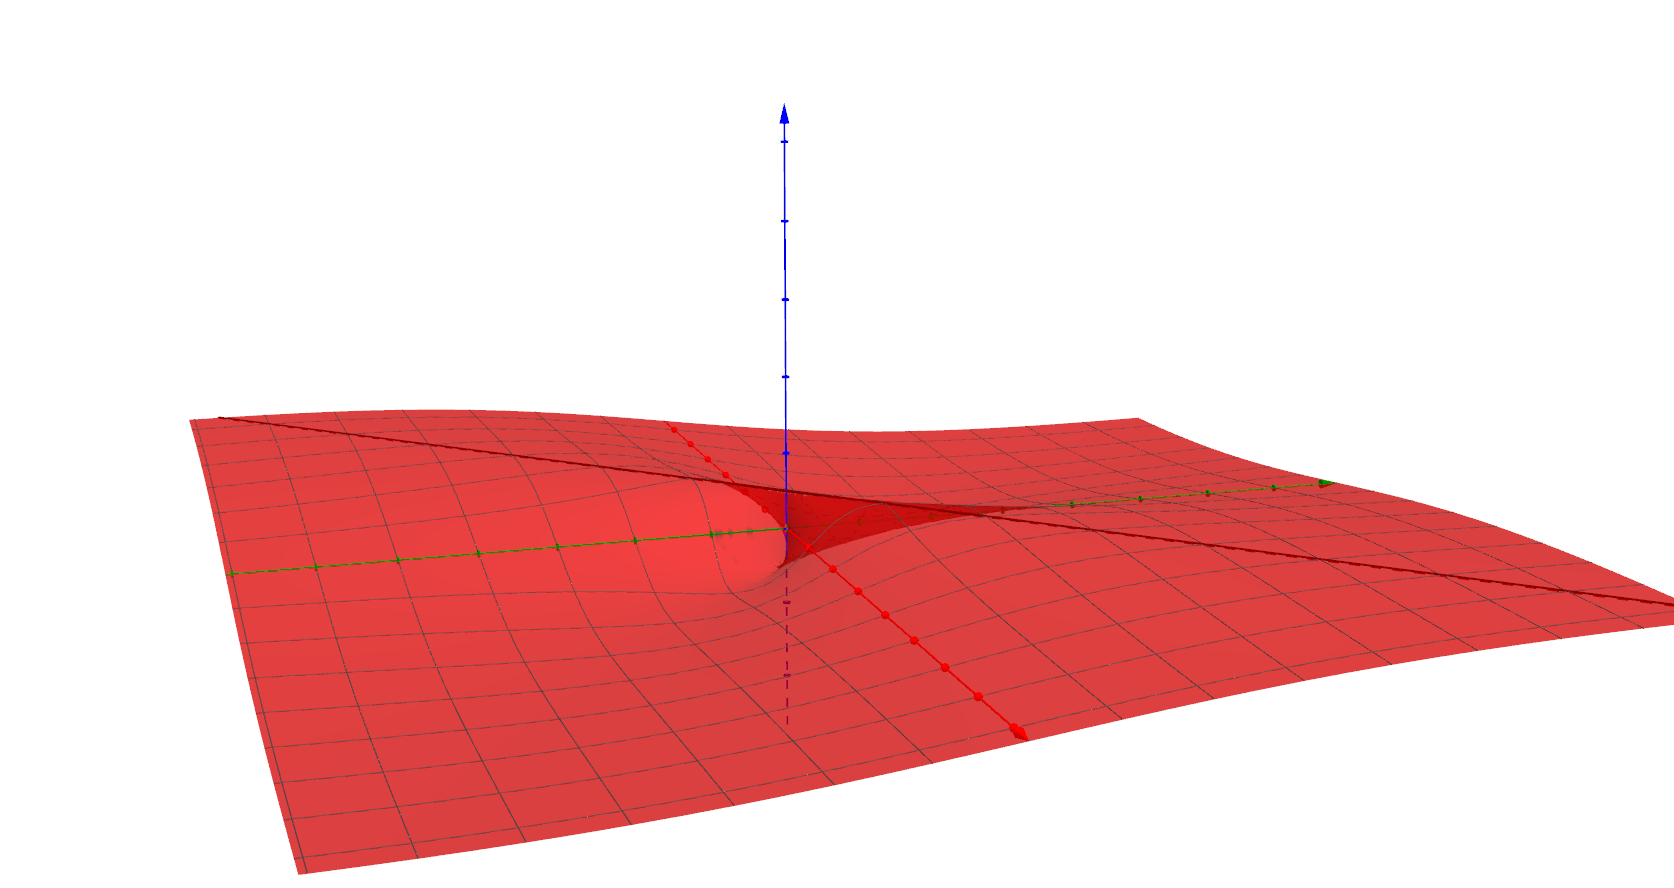
\includegraphics[width=550pt]{Continue_sur_chaque_variable}
			\caption{$\left(x, y, \frac{xy}{x^2+y^2}\right)$ et $(t, t, f(t, t))$}
		\end{figure}
\end{myrem}

\part{Compacité et complétude}

\section{Sous-suites et compacité}
	
\begin{mythm}{Bolzano-Weierstrass}

	Toute suite réelle bornée admet une sous-suite convergente.
\end{mythm}

\begin{myproof}
	Soit $(x_n)_n$ bornée par $M > 0$, on définit pour tout $n \geqslant 0$ l'ensemble $Y_n = \{x_k ~ | ~ k \geqslant n\}$ et $y_n=\sup Y_n$.
	
	On a alors pour tout $n$, $Y_{n+1} \subseteq Y_n$ et donc $y_{n+1} \leqslant y_n$.
	
	$(y_n)_n$ est donc une suite minorée par $-M$ décroissante, elle converge ainsi vers une limite $\ell = \inf \{y_n ~ | ~ n \geqslant 0\}$.
	
	Construisons une suite $(x_{k_n})_n$ à l'aide d'une suite strictement croissante $(k_n)_n$ d'entiers tels que :
	
	$$\forall n \geqslant 1, ~ |x_{k_n}-\ell| \leqslant \frac{1}{n}$$
	
	On choisit $k_0 = 1$ et on suppose avoir construit : $k_0, k_1, k_2, ..., k_{n-1}$.
	
	Par définition de la suite $(y_n)_n$, il existe un entier $p_n$ tel que : $$0 \leqslant y_{p_n} - \ell \leqslant \frac{1}{n}$$
	
	Mais $(y_k)_k$ est décroissante, alors $\forall k \geqslant p_n$ on a $0 \leqslant y_k - \ell \leqslant \frac{1}{n}$.
	
	$y_{p_n}$ étant une borne supérieure, il existe $k_n \geqslant p_n$ tel que $y_{p_n} - \frac{1}{n} \leqslant x_{k_n} \leqslant y_{p_n}$, ce qui donne :
	$$y_{p_n} - \ell - \frac{1}{n} \leqslant x_{k_n} - \ell \leqslant y_{p_n} - \ell$$
	
	En particulier on a : $$-\frac{1}{n}\leqslant x_{k_n}-\ell \leqslant \frac{1}{n}$$.
	
	\cqfd
\end{myproof}

\begin{mydef}
	Une partie de $X$ d'un espace vectoriel normé est \textit{compacte} si toute suite à valeurs dans $X$ admet une sous-suite convergente dans $X$.
\end{mydef}

\begin{myexmpl}
	Toute partie finie d'un espace vectoriel normé est compacte.
\end{myexmpl}

\begin{myproposition}
	Toute partie compacte d'un espace vectoriel normé $E$ est fermée et bornée.
\end{myproposition}

\begin{myproof}
	Soit $X$ une partie compacte de $E$.
	
	\begin{proofpart}{$X$ est fermée}
		Soit $(x_n)_n$ une suite de $X$ convergeant vers $\ell$.
		
		Comme $X$ est compact, $(x_n)_n$ admet une sous-suite convergente dans $X$, donc la limite de $(x_n)_n$ appartient à $X$.
	\end{proofpart}
	
	\begin{proofpart}{$X$ est bornée}
		Sinon il existe une suite non-bornée dans $X$ dont aucune sous-suite ne converge.
	\end{proofpart}
	
	\cqfd
\end{myproof}

\begin{myrem}
	La réciproque est fausse en général.
\end{myrem}

\begin{myproposition}
	Si $E$ est de dimension finie, les compacts de $E$ sont les fermés bornés.
\end{myproposition}

\begin{myproof}
	Soit $F \subseteq E$ un fermé borné et $(x_n)_n$ une suite à valeur dans $F$.
	
	$F$ est borné, donc $(x_n)_n$ l'est aussi, or par la généralisation du théorème de Bolzano-Weierstrass en dimension finie, $(x_n)_n$ admet une sous-suite $(y_n)_n$ convergente vers un élément $y$.
	
	Or $F$ est fermé, donc $y \in F$.
	
	$F$ est bien compact.
	
	\cqfd
\end{myproof}

\begin{myproposition}
	Soit $E$ et $F$ deux espaces vectoriels normés, $X$ une partie de $E$ et $f$ une application continue de $X$ dans $F$.
	
	Si $X$ est un compact de $E$ alors $f(X)$ est un compact de $F$.
\end{myproposition}

\begin{myrem}
	L'image réciproque d'un compact n'est pas nécessairement un compact, par exemple $sin^{-1}([0, 1])= \mathbb{R}$ et pour l'application $\func{f}{\mathbb{R}}{\mathbb{R}}{x}{1}$ on a  $f^{-1}(\{1\})=\mathbb{R}$
\end{myrem}

\begin{myproof}
	Soit $X$ un compact de $E$ et $(y_n)_n$ une suite de $f(X)$, soit alors $(x_n)_n$ tel que $y_n=f(x_n)$, qui est une suite de $X$.
	
	Comme $X$ est compact, on peut extraire une sous-suite convergente de $(x_n)$ de limite $\ell \in X$.
	
	Par continuité de $f$, la suite $(y_n)_n$ converge vers $f(\ell)$ et comme $f(\ell) \in f(X)$, on a bien que $f(X)$ est compact.
	
	
	\cqfd
\end{myproof}

\begin{mycor}
	Soit $\funcshort{f}{\mathbb{R}}{\mathbb{R}}$ une application continue avec $X$ compact de $E$, alors $f$ est bornée et atteint ses bornes.
\end{mycor}

\section{Compacité en dimension finie}

\begin{mylemma}
	Soit $E$ un espace vectoriel normé de dimension finie $d$.
	
	Soit $(e_i)_{i \leqslant d}$ une base de $E$ et soit la norme sur $E$
	
	$$\|x\|_{\infty} = \sup\limits_{1 \leqslant i \leqslant d} |x_i| ~ \text{où} ~ x = \sum_{i=1}^{d} x_i e_i$$
	
	Alors toute partie $K$ compacte de $E$ est incluse dans un ensemble de la forme : $$\left\{ \sum_{i =1}^{d} x_i e_i ~ | ~ x_i \in [a_i, b_i] \right\}$$.
\end{mylemma}

\begin{mylemma}
	Soit $E$ un espace vectoriel de dimension finie $d$ de base $e=(e_i)_{i \leqslant d}$.
	
	Alors les parties compactes de $E$ pour la norme $\|\cdot\|_{\infty}$ sont les parties fermées bornées pour cette norme dans $\mathbb{R}^d$.
\end{mylemma}

\begin{myproof}
	Soit $X$ un fermé borné de $E$, alors $X$ est inclus dans un ensemble de la forme $K = \left\{ \sum_{i =1}^{d} x_i e_i ~ | ~ x_i \in [a_i, b_i] \right\}$.
	
	Montrons que $X$ est compact.
	 Soit $(x_n)_n$ une suite de $X$, alors $(x_n)_n$ est une suite de $K$ qui est un compact, donc $(x_n)$ possède une sous-suite convergente dans $K$ et comme $X$ est fermé, sa limite est dans $X$.
	 
	 \cqfd
\end{myproof}

\begin{mycor}
	Tout sous-ensemble fermé d'un compact est compact.
\end{mycor}

\begin{mythm}
	Soit $E$ un espace vectoriel de dimension finie $d$, toutes les normes sur $E$ sont équivalentes.
\end{mythm}

\begin{myproof}
	Soit $E$ de base $e=(e_i)_{i \leqslant n}$
	
	Soit $N$ une norme sur $E$ et $\|x\|_{\infty}$ définie pour tout $x=x_1 +e_1 + ... + x_d e_d$ par $\|x\|_{\infty} = \sup\limits_i |x_i|$
	
	\begin{proofpart}{$N(x) \leqslant C_2 \|x\|_\infty$}
		Soit $x \in E$, on a :
		
		$$N(x) = N\left(\sum_{i} x_i e_i\right)$$

		$$N(x) \leqslant \sum_{i} N(x_i e_i)$$

		$$N(x) \leqslant \sum_{i} |x_i| N(e_i)$$

		$$N(x) \leqslant \sum_{i} |x_i| \leqslant C_2 \|x\|_{\infty}$$
		
		avec $C_2 = \sum_i N(e_i)$
	\end{proofpart}
	
	\begin{proofpart}{$\|x\|_\infty \leqslant \beta N(x)$}
		Par l'inégalité triangulaire, on a $|N(x)-N(y)| \leqslant N(x-y)$ et d'après l'étape précédente, $|N(x) - N(y)| \leqslant C_2 \|x-y\|_{\infty}$, $N$ est donc continue sur $E$.
		
		Comme la sphère unité $\mathcal{S}_1^{\infty}$ est compacte (car bornée et fermé dans $E$) $N_{|\mathcal{S}_1^{\infty}}$ est continue et $N_{|\mathcal{S}_1^{\infty}}(\mathcal{S}_1^{\infty})$ est bornée, il existe donc un $x_0$ tel que $\forall x \in S^{\infty}_1, N(x) \geqslant N(x_0)$.
		
		On pose $C_1=N(x_0)$ et on a :
		
		$$\forall x \in E, ~ N(x) = \|x\|_{\infty} \cdot  N\left(\frac{x}{\|x\|_{\infty}}\right) \geqslant C_1 \|x\|_{\infty}$$.
	\end{proofpart}
	
	\cqfd
\end{myproof}

\begin{mythm}
	Soient $E$ et $F$ des espaces vectoriels normés de dimension finie, et $\funcshort{\varphi}{E}{F}$.
	
	Si $\varphi$ est linéaire, alors elle continue.
\end{mythm}

\begin{myproof}
	Soit $e$ une base de $E$ et $\|\cdot\|_{\infty}$ la norme associée.
	
	Soit $N$ une norme sur $F$ et $x \in E$.
	
	$$N(\varphi(x))=N\left(\varphi \left(\sum_{i} x_i e_i\right)\right)$$

	$$N(\varphi(x))=N\left(\sum_{i} x_i \varphi \left(e_i\right)\right)$$
	
	$$N(\varphi(x))= \sum_{i} |x_i| N\left(\varphi \left(e_i\right)\right)$$
	
	$$N(\varphi(x)) \leqslant \|x\|_{\infty} \sum_i N(\varphi (e_i))$$
	
	$\varphi$ est donc bien continue.
\end{myproof}

\section{Applications de la compacité}

\begin{mythm}
	Soient $E$ et $F$ deux espaces vectoriels normées et $K$ un compact de $E$.
	
	Alors toute application $\funcshort{f}{K}{F}$ continue est uniformément continue.
\end{mythm}

\begin{myproof}
	Supposons que $f$ n'est pas uniformément continue, alors il existe $\varepsilon > 0$ tel que pour tout $\delta > 0$, il existe $x$ et $y$ dans $K$ tels que $\|x-y\| \leqslant \delta$ et $\|f(x) - f(y)\| \geqslant \varepsilon$.
	
	En particulier, pour tout $n > 0$, il existe $x_n$ et $y_n$ dans $K$ tels que $\|x_n-y_n\| \leqslant \frac{1}{n}$ et $\|f(x_n) - f(y_n)\| \geqslant \varepsilon$.
	
	Alors $(x_n)_n$ possède une sous-suite $(x_{\varphi(n)})_n$ convergente dans $K$ vers une limite $x \in K$.
	
	De même pour $(y_{\varphi(n)})$ qui possède une sous-suite $(y_{(\varphi \circ \psi)(n)})$ qui converge vers une limite $y \in K$.
	
	Soient $x'_n = x_{(\varphi \circ \psi)(n)}$ et $y'_n = y_{(\varphi \circ \psi)(n)}$.
	
	Alors $\|x'_n - y'_n\| \leqslant \frac{1}{(\varphi \circ \psi)(n)} \leqslant \frac{1}{n}$.
	
	Donc $x=y$, mais $f$ est continue en $x$, donc $f(x'_n)$ converge vers $f(x)$ et $f(y'_n)$ converge vers $f(x)$, ce qui est contradictoire avec le fait que $\|f(x'_n) - f(y'_n)\| \geqslant \varepsilon$.
\end{myproof}

\section{Suites de Cauchy}

\begin{mydef}
	Une suite $(x_n)_n$ est dite \textit{de Cauchy} si : $$\forall \varepsilon > 0, ~ \exists N ~ : ~ \forall m, n \in \mathbb{N}, ~(m, n \geqslant N \Longrightarrow \|x_m - x_n\| \leqslant \varepsilon)$$
	et de manière équivalente :
	$$\forall \varepsilon > 0, ~ \exists N ~ : ~ \forall m, n \in \mathbb{N}, ~(m \geqslant N \Longrightarrow \|x_m - x_{m+n}\| \leqslant \varepsilon)$$
\end{mydef}

\begin{myrem}
	Une définition équivalente d'une suite de Cauchy est une suite $(x_n)_n$ telle que $\delta(A_k) \longrightarrow 0, ~ (k \rightarrow \infty)$ où $A_k = \{x_n |n \geqslant k\}$ et $\delta (X) = \sup\limits_{x, y \in X} \|x - y\|$.
\end{myrem}

\begin{myproposition}
	Soit $\funcshort{f}{E}{F}$ une application uniformément continue sur $E$, si $(x_n)_n$ est une suite de Cauchy de $E$, alors $(f(x_n))_n$ est une suite de Cauchy de $F$.
\end{myproposition}

\begin{myproof}
	Il s'agit de vérifier que pour tout $\varepsilon > 0$, il existe $N$ tel que pour tous $m, n > N$ on a $\|f(x_n)-f(x_m)\| \leqslant \varepsilon$.
	
	Soit $\varepsilon > 0$, il existe $\delta > 0$ tel que pour tous $x, y \in E$, on a $\|x-y\| < \delta \Longrightarrow \|f(x)-f(y)\| < \varepsilon$.
	
	Comme $(x_n)_n$ est de Cauchy, il existe $N$ tel que si $m, n > N$ alors $\|x_m - x_n\| < \delta$ et par suite $\|f(x_m)-f(x_n)\| < \varepsilon$.
	
	\cqfd
\end{myproof}

\begin{myproposition}
	Soit $E$ un espace vectoriel normé.
	
	\begin{enumerate}
		\item Toute suite de Cauchy est bornée.
		\item Toute suite convergente est de Cauchy.
		\item Toute sous-suite d'une suite de Cauchy est de Cauchy.
		\item Si une suite de Cauchy admet une sous-suite convergente, alors elle converge.
	\end{enumerate}
\end{myproposition}

\begin{myproof}
	\begin{proofpart}{Point 1}
		Soit $N$ tel que pour tout $n \geqslant N$, on ait $\|x_n - x_N\| < 1$, alors $\|x_n\| - \|x_N\|< 1$ d'où $\|x_n\| < 1 + \|x_N\|$
		et donc $\|x_n\| \leqslant \max (\|x_0\|, ..., \|x_{N-1}\|, 1 + \|x_N\|)$
	\end{proofpart}
	
	\begin{proofpart}{Point 4}
		On suppose qu'il existe une sous-suite convergente $(x_{\varphi(n)})_n$ convergente vers une limite $\ell$.
		
		Soit $\varepsilon > 0$, il existe $N$ et $N'$ tels que : $$\forall n \geqslant N, ~ \|x_{\varphi(n)} - \ell\| \leqslant \frac{\varepsilon}{2}$$
		et :
		$$\forall n, m \geqslant N' ~ \|x_n - x_m\| \leqslant \frac{\varepsilon}{2}$$
		
		On note $N_0 = \max (N, N')$, si $m \geqslant N_0$ et $n \geqslant N_0$, alors $\|x_m - \ell\| \leqslant \|x_m - x_{\varphi(n)}\| + \|x_{\varphi(n)} - \ell\| \leqslant \varepsilon$.
	\end{proofpart}
\end{myproof}

\begin{mycor}
	Dans un compact, toute suite de Cauchy est convergente.
\end{mycor}

\begin{myrem}
	En dimension infini, les parties fermées et bornées ne sont pas forcément compactes.
	
	Soit $E$ l'ensemble des polynômes sur $\mathbb{R}$ muni de la norme :
	$$\|P\| = \sum_{i=0}^{n} |a_i|, \text{ avec } n \text{ le degré de } P$$
	
	Soit la suite $(P_n)_n = (X^n)_n$, alors pour tout $n$, $\|P_n\|=1$
	
	$(P_n)_n$ est une suite de $\mathcal{B}_1$, or celle-ci est bornée et fermée dans $E$, mais $\|P_n-P_m\| = 2$ si $n \neq m$.
	
	Donc $(P_n)_n$ n'est pas de Cauchy, et n'admet aucune sous-suite convergente. $\mathcal{B}_1$ n'est donc pas de Cauchy.
\end{myrem}

\section{Parties complètes et espaces de Banach}

\begin{mydef}
	On dit qu'une partie $X$ d'un espace vectoriel normé $E$ est \textit{complète} si toute suite de Cauchy dans $X$ converge dans $X$. On dit aussi que $X$ est complet.
\end{mydef}

\begin{myproposition}
	\leavevmode
	\begin{enumerate}
		\item Toute partie compacte est complète.
		\item Tout espace vectoriel de dimension finie est complet.
		\item Toute partie complète d'un espace vectoriel normé est fermée.
		\item Toute partie fermée d'un complet est complète.
	\end{enumerate}
\end{myproposition}

\begin{myproof}
	\begin{proofpart}{Point 2}
		Soit $(x_n)_n$ une suite de Cauchy de $E$ de dimension finie, alors elle est bornée, donc elle admet une sous-suite convergente (car $E$ est de dimension finie), et donc $(x_n)_n$ converge.
	\end{proofpart}
	
	\begin{proofpart}{Point 3}
		Soit $(x_n)_n$ une suite convergente de $X$ complet, montrons que la limite $\ell$ de $(x_n)_n$ est dans $X$.
		
		$(x_n)_n$ est convergente donc elle est de Cauchy. Comme $X$ est complet $(x_n)_n$ converge dans $X$, d'où le résultat par unicité de la limite.
	\end{proofpart}
	
	\begin{proofpart}{Point 4}
		Soit $F$ un ensemble fermé de $X$ complet, montrons que $F$ est complet.
		
		Soit $(x_n)_n$ une suite de Cauchy de $F$ montrons que $(x_n)_n$ converge dans $F$.
		
		Comme $F \subseteq X$ qui est complet alors $(x_n)_n$ converge dans $X$.
		
		Comme $F$ est fermé et que $(x_n)_n$ converge, sa limite est dans $F$.
	\end{proofpart}
\end{myproof}

\begin{mydef}
	Si $E$ est un espace vectoriel normé complet alors on dit que $E$ est un \textit{espace de Banach}.
\end{mydef}

\begin{myexmpl}
	$\mathbb{R}, \mathbb{R}^n, \mathbb{R}_n[X], \text{Mat}_{n \times m}(\mathbb{R}), \mathbb{C}$ sont complets.
	
	\begin{enumerate}
		\item $\mathbb{Q}$ n'est pas complet (dans $\mathbb{R}$).

		Considérons la suite $$x_0, ~ x_{n+1} = 1 + \frac{1}{x_n}$$
		
		$(x_n)_n$ est bornée par 1 et 2, elle admet donc une sous-suite convergente convergente dans $\mathbb{R}$ de limite $\ell$ vérifiant $\ell = 1 + \frac{1}{\ell}$, donc $\ell = \frac{1+\sqrt{5}}{2}$.
	\end{enumerate}
\end{myexmpl}

On rappelle qu'une série $\sum x_n$ est normalement convergente si $\left(\sum \|x_n\|\right)_n$ est convergente.

\begin{myproposition}
	Soit $E$ un espace vectoriel normé, alors $E$ est de Banach si et seulement si toute série normalement convergente est convergente.
\end{myproposition}

\begin{myproof}
	\begin{proofpart}{$\Longrightarrow$}
	Soit $(x_n)_n$ telle que $\sum x_n$ soit normalement convergente.
	
	On note $\displaystyle S_n = \sum_{i = 0}^{n} x_n$ et on montre que $(S_n)_n$ converge dans $E$.
	
	Soient $n > m$, alors $\displaystyle S_n - S_m = \sum_{i = m + 1}^{n} x_i$ et donc $\displaystyle \|S_n - S_m\| \leqslant \sum_{i = m+1}^{n} \|x_i\| \leqslant \sum_{k = m + 1}^{\infty}\|x_i\|$.
	
	Sachant que $\sum \|x_k\|$ converge, on a que $\displaystyle \sum_{i = m + 1}^{\infty} \|x_i\| \longrightarrow 0, ~ (m \rightarrow \infty)$.
	
	Donc pour tout $\varepsilon > 0$, il existe un $N$ tel que pour tout $m \geqslant N$ on a $\displaystyle \sum_{k \geqslant m+1} \|x_k\| \leqslant \varepsilon$, d'où $$\forall m \geqslant N, \forall n \geqslant 0, ~ \|S_n - S_m\| \leqslant \varepsilon$$.
	
	Donc $(S_n)_n$ est une suite de Cauchy. Comme $E$ est de Banach, elle converge.
	\end{proofpart}
	
	\begin{proofpart}{$\Longleftarrow$}
		Soit $(x_n)_n$ une suite de Cauchy dans $E$, montrons qu'elle converge dans $E$.
		
		$(x_n)_n$ étant de Cauchy, pour tout $k \geqslant 0$, il existe $N_k$ tel que pour tout$n, m \geqslant N_k$ on a $\|x_n - x_m\| \leqslant 2^{-k}$
		
		On pose $y_k = x_{N_{k+1}} - x_{N_k}$, alors $\|y_k\| \leqslant 2^{-k}$ donc $\displaystyle \sum_{k \geqslant 0} \|y_k\|$ converge.
		
		Mais alors $\sum_{k \geqslant 0} y_k$ converge dans $E$ par hypothèse.
		
		On écrit alors : $$\sum_{i = 0}^{k} y_i = y_0 + y_1 + ... + y_k$$
		
		$$\sum_{i = 0}^{k} y_i = x_{N_{k+1}} - x_{N_0}$$
		
		Donc $\displaystyle X_{N_{k+1}} = x_{N_0} + \sum_{i=0}^k y_i$ , alors $(x_n)_n$ admet une sous-suite convergente, donc ele converge.
	\end{proofpart}

	\cqfd
\end{myproof}

\begin{myproposition}
	Une partie de $X$ d'un espace vectoriel normé $E$ est complète si et seulement si toute suite décroissante de fermés non-vides de $E$, dont le diamètre tend vers 0 a une intersection non-vide.
\end{myproposition}

\begin{myproof}
	\begin{proofpart}{$\Longrightarrow$}
		Soit $X \subseteq E$ complet et une suite $(F_n)_n$ telle que :
		
		$$
		\left\{
			\begin{array}{l}
				\forall n, ~ F_n \neq \emptyset \\
				\forall n, ~ F_{n+1} \subseteq F_n \\
				\delta (F_n) \longrightarrow 0, ~ (n \rightarrow 0) \\
			\end{array}
		\right.
		$$
		
		Pour tout $n$, on choisit un élément $x$ de $F_n$, cette suite est de Cauchy car le diamètre des $F_n$ tend vers 0 : en effet si $n > m$, alors $x_n \in F_n$ et $\|x_n - x_m\| \leqslant \delta (F_m)$.
		
		Mais alors $(x_n)_n$ converge dans $X$, puisque $X$ est complet.
		
		Soit $x$ sa limite, montrons que $x \in \bigcap_{n \geqslant 0} F_n$.
		
		Soit $m$ et soit la suite $(x_n)_{n \geqslant m}$. Cette suite converge vers $x$ et par ailleurs c'est une suite de $F_m$.
		
		Comme $F_m$ est fermé, on a $x \in F_m$, d'où $x \in \bigcap_{m \geqslant 0} F_m = \bigcap_{m \geqslant 0} F_m$
		
		C'est d'ailleurs l'unique élément de l'intersection puisque $\delta(F_n) \longrightarrow 0 ~ (n \rightarrow \infty))$
	\end{proofpart}
	
	\begin{proofpart}{$\Longleftarrow$}
		Sot $(x_n)_n$ une suite de Cauchy de $X$, montrons que $(x_n)_n$ converge dans $X$.
		
		Pour tout $m$ on définit le fermé $F_m=\overline{\{x_n | n \geqslant m\}}$.
		
		Alors la famille des $F_m$ est décroissante, les fermés sont non-vides et $\delta(F_m) \longrightarrow 0 ~ (m \rightarrow \infty)$ car $(x_n)_n$ est de Cauchy.
		
		L'intersection des $F_m$ est formée de l'ensemble des valeurs d'adhérence de la suite $(x_n)$, par hypothèse cet ensemble est non-vide, donc $(x_n)_n$ possède au moins une sous-suite convergente, donc $(x_n)_n$ converge car elle est de Cauchy.
	\end{proofpart}
	
	\cqfd
\end{myproof}

\begin{mythm}
	Soit $A$ un ensemble et $X$ une partie complète d'un espace vectoriel normé $E$, alors :
	\begin{enumerate}
		\item $\mathcal{F}_b(A, X)$ est un espace de Banach s'il est muni de la norme uniforme.
		
		\item Si de plus $A$ est compact, alors l'ensemble $\mathcal{C}(A, X)$ des fonctions continues de $A$ dans $X$ est un espace de Banach.
	\end{enumerate}
\end{mythm}

\begin{myproof}
	\begin{proofpart}{Point 1}
		Soit $(f_n)$ une suite de Cauchy de $\mathcal{F}_b(A, X)$, alors pour tout $\varepsilon > 0$ il existe $N$ tel que pour tous $mn , \geqslant N$, on a $\|f_n - f_m\| \leqslant \varepsilon$.
		
		Alors en particulier pour tout $x \in A, ~ \|f_n(x) - f_m(x)\| < \varepsilon$, donc pour tout $x \in A$ la suite $(f_n(x))_n$ est de Cauchy dans $X$, donc elle converge vers une limite $f(x)$ car $X$ est complet.
		
		Il faut vérifier que $f \in \mathcal{F}_b(A, X)$.
		
		On reprend $\|f_n(x) - f_m(x)\| < \varepsilon$ pour passer à la limite $n \rightarrow \infty$ avec $m > N$ fixé, alors $\|f(x)-f_m(x)\| < \varepsilon$ et donc $\|f(x)\| < \varepsilon + \|f_n(x)\|$.
		
		Donc $f \in \mathcal{F}_b(A, X)$ avec $\|f\| \leqslant \varepsilon + \|f_m\|$.
		
		Enfin il faut vérifier que $\lim\limits_{m \to \infty} \|f_m - f\| = 0$, ce qui est vrai car $\sup_x \|f(x) - f_m(x)\| \leqslant \varepsilon$ dès que $m > N$.
	\end{proofpart}
	
	\begin{proofpart}{Point 2}
		On remarque que $\mathcal{C}(A, X) \subseteq \mathcal{F}_b(A, X)$ car $A$ est compact.
		
		Donc il suffit de montrer que $\mathcal{C}(A, X)$ est fermé pour la norme uniforme, ce qui est vrai par la limite uniforme de fonctions continues.
	\end{proofpart}
	
	\cqfd
\end{myproof}

\begin{mythm}
	Soient $E$ et $F$ deux espaces vectoriels normés avec $F$ complet, alors l'ensemble $\mathcal{L}_c(E, F)$ des applications linéaires continues de $E$ dans $F$ munie de la norme d'opérateur est un espace de Banach.
\end{mythm}

\begin{myproof}
	On sait que $\mathcal{L}_c(E, F)$ est un espace vectoriel normé, il ne reste qu'à démontrer qu'il est complet.
	
	Soit $(u_n)_n$ une suite de Cauchy à valeur dans $\mathcal{L}_c(E, F)$, montrons qu'elle converge vers un élément $u$ de $\mathcal{L}_c(E, F)$.
	
	On sait que :
	
	$$\forall \varepsilon > 0, ~ \exists N ~ : ~ \forall n,m, ~ (n,m \geqslant N \Longrightarrow ~ \|u_n - u_m\| \leqslant \varepsilon)$$
	
	Ce qui veut dire que $$\sup_{\|x\| \leqslant 1} \|u_n(x) - u_m(x)\| \leqslant \varepsilon$$ Donc pour tout $x$, $(u_n(x))_n$ est une suite de Cauchy, et sachant $F$ complet on peut poser $u(x)=\lim\limits_{n} u_n (x)$.
	
	Il reste à démontrer que $u$ est une application linéaire et que : $$\lim\limits_{n} \|u_n - u\| = 0$$
	ce qui impliquera entre autre la continuité de $u$.
	
	\begin{itemize}
		\item Soient $x, y \in E$ et $\lambda \in \mathbb{R}$, $u_n$ est linéaire alors par passage à la limite :
		$$u_n(x+\lambda y) = u_n(x) + \lambda u_n(y) \longrightarrow u(x) + \lambda u(y) ~ (n \rightarrow \infty)$$
		
		\item En passant à la limite en $m$, on obtient :
		
		$$\forall \varepsilon > 0, \exists N ~ : ~ (n \geqslant N \Longrightarrow \sup_{\|x\| \leqslant 1}\|u_n(x)-u(x)\| \leqslant \varepsilon)$$
		
		Ainsi $\lim\limits_{n} \|u_n - u\| = 0$, et de plus elle est bornée grâce au théorème précédent.
	\end{itemize}
\end{myproof}

\section{Applications}

\begin{mythm} Théorème de Riesz
	
	Soit $E$ un espace vectoriel normé, alors $E$ est de dimension fini si et seulement si la boule unité fermée de $E$ est compacte.
\end{mythm}

\begin{myproof}
	Montrons que si la boule unité fermée est compacte, alors $E$ est de dimension finie.
	
	Supposons par l'absurde que $E$ de dimension infinie et que sa boule unité fermée $B$ soit compacte.
	
	On construira par récurrence une suite $(x_n)_n$ de Cauchy de $B$ telle que $\|x_n - x_m\| \geqslant \frac{1}{2}$, ce qui contredira le fait que la boule unité fermée soit compacte car cette suite ne possède aucune sous-suite convergente.
	
	On pose $x_0 = 0$ et on suppose construits $x_0, ..., x_n$ dans $B$ tels que $\|x_i - x_j\| \geqslant \frac{1}{2}$ pour tous $i, j \leqslant n$.
	
	Soit $F_n = \text{Vect}(x_0, x_1, ..., x_n)$, alors $\dim F_n \leqslant n+1$, sachant $E$ de dimension infinie, il existe un élément $a \in E \backslash F_n$.
	
	On note $d(a, F_n) = \min_{f \in F_n} \|a-f\|$, et soit $b$ tel que $\|a-b\| \leqslant 2 \cdot d(a, F_n)$.
	
	Posons $x_{n+1} = \frac{a-b}{\|a-b\|}$, alors $x_{n+1} \in B$.
	
	Il reste à vérifier que : $\forall k \leqslant n, ~ \|x_{n+1} - x_k\| \geqslant \frac{1}{2}$
	
	On remarque que $d(a, F_n)=d(a-b, F_n)$, en effet : $$d(a-b, F_n) = \min_{f \in F_n} \|a-b-f\| = \min_{f \in F_n} \|a-(b+f)\| = \min_{b+f \in F_n} \|a-(b+f)\| = \min_{f' \in F_n} \|a-f'\|$$
	
	De même $d(\frac{a-b}{\|a-b\|}, F_n) = \frac{d(a-b, F_n)}{\|a-b\|}$.
	
	Donc $d(x_{n+1}, F_n) = \frac{1}{\|a-b\|}d(a-b, F_n) = \frac{1}{\|a-b\|}d(a, F_n) \geqslant \frac{1}{\|a-b\|} \cdot \frac{\|a-b\|}{2} \geqslant \frac{1}{2}$
	
	Enfin on a $\forall k \leqslant n, ~ d(x_n, F_n) \leqslant \|x_{n+1} - x_k\|$
\end{myproof}

\begin{mythm}Théorème du point fixe

	Soit $E$ un espace vectoriel normé et $X$ une partie complète de $E$ non-vide.
	
	Soit $\funcshort{f}{X}{X}$ un application contractante, c'est-à-dire $k$-Lipschitzienne avec $0 < k < 1$, alors :
	\begin{enumerate}
		\item $f$ possède un unique point fixe $z_0$
		\item pour tout point $x \in X$, la suite définie par
		$$\left\{
			\begin{array}{l}
				x_0 = x \\
				x_{n+1} = f(x_n), ~ n \geqslant 0
			\end{array}
		\right.$$
		
		converge vers $z_0$.
	\end{enumerate}
\end{mythm}

\begin{myproof}
	Soit $x \in X$ et la suite $(x_n)_n$ définie par :
	
	$$\left\{
		\begin{array}{l}
			x_0 = x \\
			x_{n+1} = f(x_n), ~ n \geqslant 0
		\end{array}
	\right.$$
	
	Montrons que cette suite converge.
	
	Comme $X$ est complet, il suffit de vérifier que $(x_n)_n$ est de Cauchy :
	
	$$\|x_{n+1} - x_n\| = \|f(x_n) - f(x_{n-1})\|$$
	
	$$\|x_{n+1} - x_n\| \leqslant k \cdot\|x_n - x_{n-1}\| = k \cdot \|f(x_{n-1}) - f(x_{n-2})\|$$
	
	$$\|x_{n+1} - x_n\| \leqslant k \cdot \|f(x_{n-1}) - f(x_{n-2})\| = k^2 \cdot \|x_{n-1} - x_{n-2}\|$$
	
	$$...$$
	
	$$\|x_{n+1}-x_n\| \leqslant k^n \|x_1 - x_0\|$$
	
	Soient $n$ et $m$, on a : $$\|x_{n+m} - x_n\| = \|x_{n+m} - x_{n+m-1} + x_{n+m-1} ... + x_{n+1} - x_n\|$$
	
	$$\|x_{n+m} - x_n\| \leqslant \sum_{j = 1}^{m} \|x_{n+j} - x_{n+j-1}\|$$
	
	$$\|x_{n+m} - x_n\| \leqslant \sum_{j = 1}^{m} k^{n+j-1}\|x_1 - x_0\| = k^n \sum_{j=1}^{\infty} k^{j-1} \|x_1 - x_0\|$$

	Donc comme $k < 1$, on a que $(x_n)_n$ est une suite de Cauchy, et $X$ étant complet on en déduite que $(x_n)_n$ converge dans $X$ vers un élément $_0 \in X$.
	
	Montrons que $f(z_0)=z_0$ puis que $z_0$ est l'unique point fixe de $f$.
	
	On sait que $x_{n+1} = f(x_n)$, comme $f$ est continue et donc par passage à la limite $z_0 = f(z_0)$.
	
	$z_0$ est de plus unique car si on a deux points fixes $z$ et $z'$, on a $\|z-z'\|=\|f(z)-f(z')\| \leqslant k \cdot \|z-z'\|$, donc nécessairement $z=z'$ car $0 < k < 1$.
	
	\cqfd
\end{myproof}

\part{Fonctions dérivables}

\section{Rappels sur les fonctions dérivables réelles}

\begin{mydef}
	Soit $f$ une fonction définie su un intervalle $I$ de $\mathbb{R}$ et à valeurs dans $\mathbb{R}$.
	
	Soi $x_0 \in I$, on dit que $f$ est dérivable en $x_0$ si :
	
	$$\lim\limits_{\substack{x \to x_0 \\ x \neq x_0}} \frac{f(x) - f(x_0)}{x - x_0}$$
	
	existe et est fini.
	
	Cette limite s'appelle la dérivée de $f$ en $x$ et se note $f'(x_0)$ ou $\frac{df}{dx}(x_0)$.
	
	La fonction $f$ est \textit{dérivable sur $I$} si elle est dérivable en tout point de $I$ et on note $f'$ ou $\frac{df}{dx}$ la fonction dérivée $x \longmapsto f'(x)$.
\end{mydef}

\begin{myproperty}
	\begin{itemize}
		\item Une fonction dérivable est continue
		\item Soient $f$ et $g$ dérivables sur un même intervalle, alors on a :
		\begin{itemize}
			\item $(f+g)'=f'+g'$
			\item $(\lambda f)'=\lambda f$
			\item $(\frac{f}{g})'=\frac{f'g-fg'}{g^2}$
			\item $(g \circ f)'=f' \cdot (g' \circ f)$
		\end{itemize}
	\end{itemize}
\end{myproperty}

\begin{myproposition}
	Soit $\funcshort{f}{I}{\mathbb{R}}$ dérivable, si $f$ admet un extremum local en $x_0$, alors $f'(x_0) = 0$.
\end{myproposition}

\begin{myproof}
	On peut supposer que $x_0$ est un maximum local, pour $h > 0$ assez petit on a $$\frac{f(x_+h_0) - f(x_0)}{h} \leqslant 0$$
	et
	$$\frac{f(x_-h_0) - f(x_0)}{h} \geqslant 0$$
	
	et en passant à la limite :
	
	$$\lim\limits_{h \to 0} \frac{f(x_+h_0) - f(x_0)}{h} = 0$$
	
	\cqfd
\end{myproof}

\begin{mythm}Théorème de Rolle
	
	Soit $\funcshort{f}{[a, b]}{\mathbb{R}}$ continue et dérivable sur $]a, b[$, s'il existe $a$ et $b$ tels que $f(a)=f(b)$ alors il existe un point $c \in ]a, b[$ tel que $f'(c)=0$.
\end{mythm}

\begin{myproof}
	$f$ est continue sur $[a,b]$ donc bornée et atteint ses bornes, on pose alors :
	
	$$m = \min_{[a, b]} f$$
	
	$$M = \max_{[a, b]} f$$
	
	et soit$x_0$ tel que $f(x_0)=m$ et $x_1$ tel que $f(x_1)=M$.
	
	Si $x_0=x_1$, c'est que la fonction est constante, et donc $\forall x \in ]a, b[f'(x)=0$, alors $m=M$.
	
	Sinon, ce sont des extremums locaux et par la proposition précédente, la dérivée s'annule en ce point.
	
	\cqfd
\end{myproof}

\begin{mythm}Théorème des accroissements finis

	Soit $\funcshort{f}{[a, b]}{\mathbb{R}}$ alors il existe $c \in [a, b]$ tel que $f(b)-f(a) = f'(c)(b-a)$
\end{mythm}

\begin{myproof}
	Appliquer le théorème de Rolle à $\phi ~ : t \longmapsto f(t) - f(a) - \frac{t-a}{b-a}(f(b)-f(a))$
\end{myproof}

\begin{mycor}
	\begin{itemize}
		\item Si $f' \geqslant 0$ alors $f$ est croissante.
		\item Si $f' \leqslant 0$ alors $f$ est décroissante. 
		\item Si $f' = 0$ alors $f$ est constante.
	\end{itemize}
\end{mycor}

\begin{mycor}
	Soit $I$ un intervalle ouvert de $\mathbb{R}$, $\funcshort{f}{I}{\mathbb{R}}$ dérivable telle que $f' > 0$.
	
	Alors $f(I)$ est ouvert, $f$ est bijective de $I$ sur $f(I)$ et $(f^{-1})'=\frac{1}{f' \circ f^{-1}}$.
\end{mycor}

\begin{myproof}
	Montrons que $f^{-1}$ est dérivable.
	
	Soit $x_0 \in I$ et $x \in I$, on pose $y=f(x)$ et $y_0=f(x_0)$.
	
	Alors si $y \longrightarrow y_0$ on a $x \longrightarrow x_0$ par continuité de $f^{-1}$.
	
	On veut calculer
	
	$$\lim\limits_{y \to y_0} \frac{f^{-1}(y) - (f^{-1})'(y_0)}{y-y_0}$$
	
	alors par $\lim\limits_{x \to x_0} \frac{(x)-f(x_0)}{x - x_0} = f'(x_0)$
	
	on a $$\lim\limits_{y \to y_0} \frac{y-y_0}{f^{-1}(y) - (f^{-1})'(y_0)} = f'(x_0)$$
		
	et comme $f'(x_0) > 0$ on a $$\lim\limits_{y \to y_0} \frac{y-y_0}{f^{-1}(y) - (f^{-1})'(y_0)} = \frac{1}{f'(x_0)} = \frac{1}{f'(f^{-1}(y_0))}$$ 
\end{myproof}

\end{document}